\documentclass[a4,12pt]{article} 
\usepackage{graphicx}
\usepackage{xepersian} 
\settextfont{Yas} 
\title{ تکالیف سری سوم کنترل خطی}
\author{یاسمین خورشیدی 40117963}
\begin{document}
	\maketitle
		
			\centering
			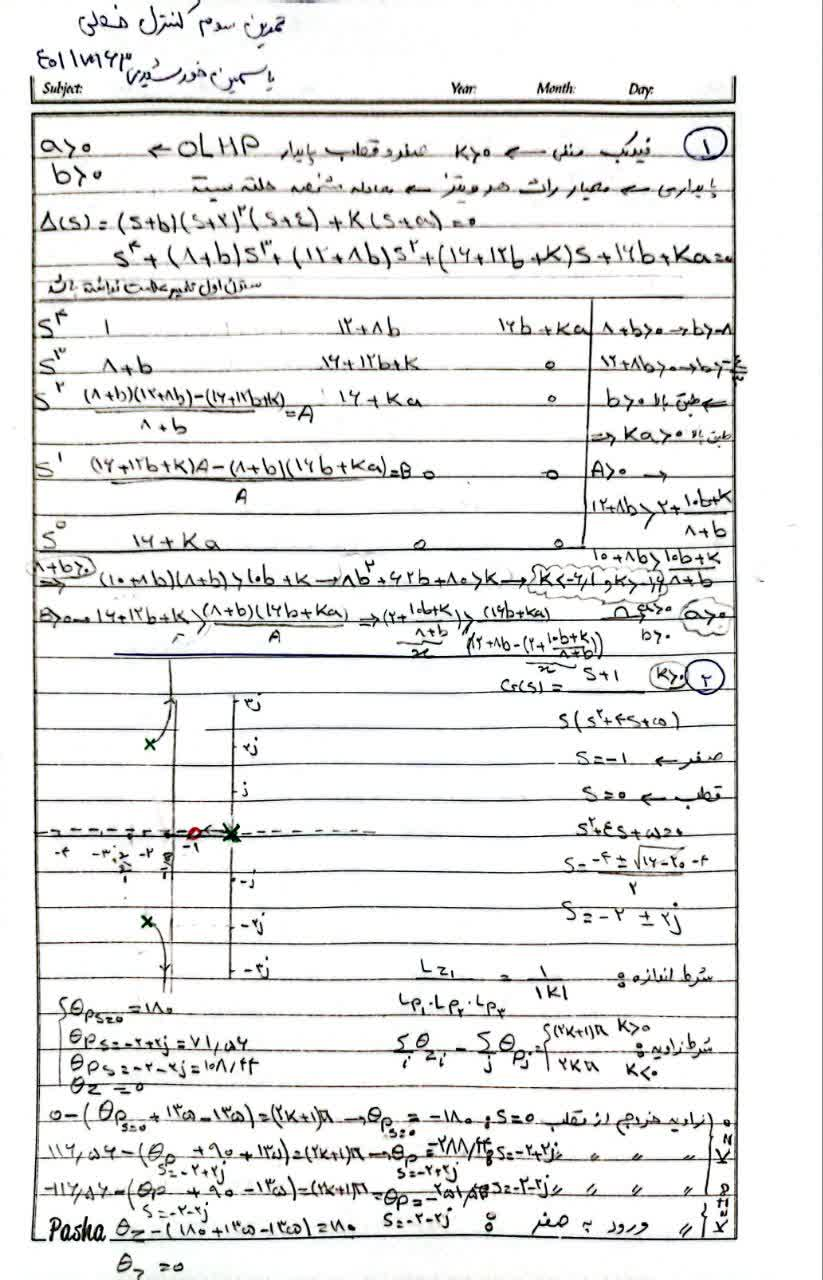
\includegraphics[width=15cm]{q1,2.jpg}
			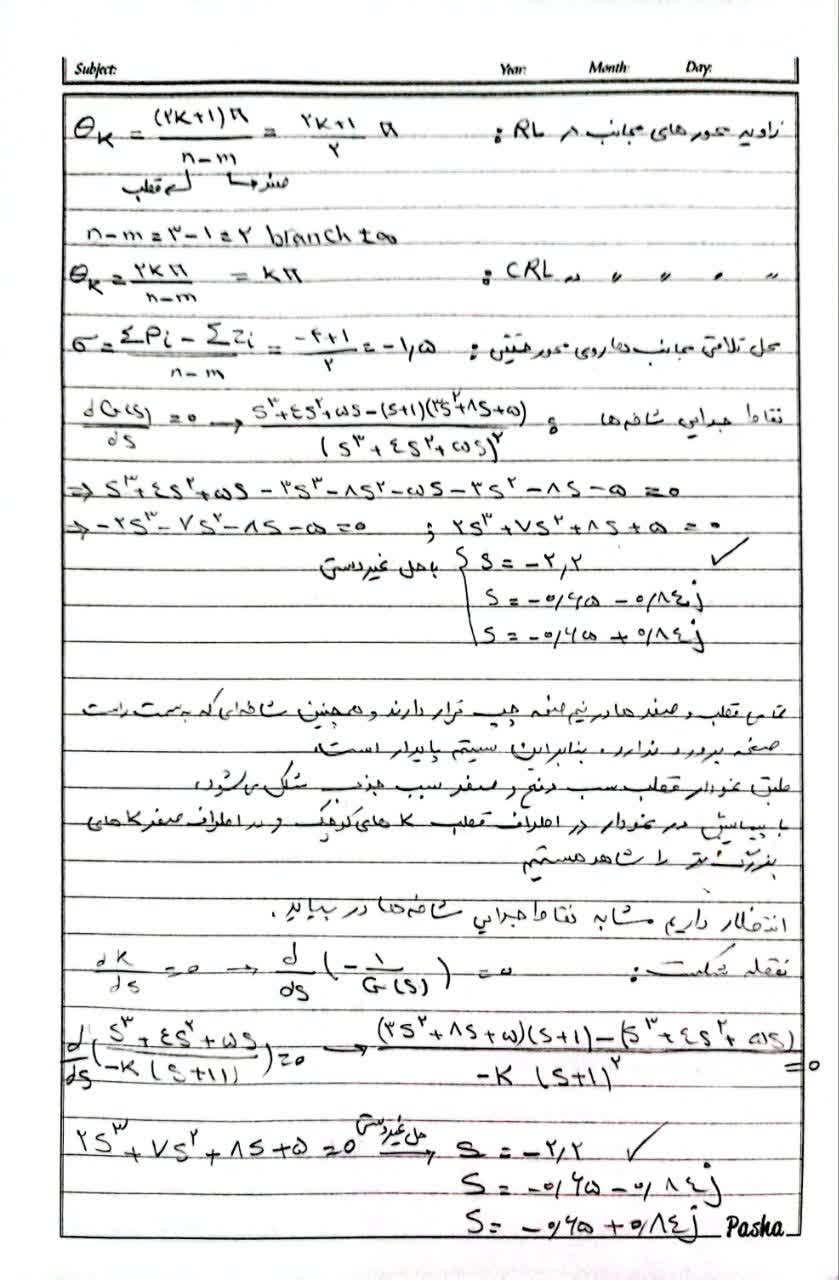
\includegraphics[width=15cm]{q2.jpg}
			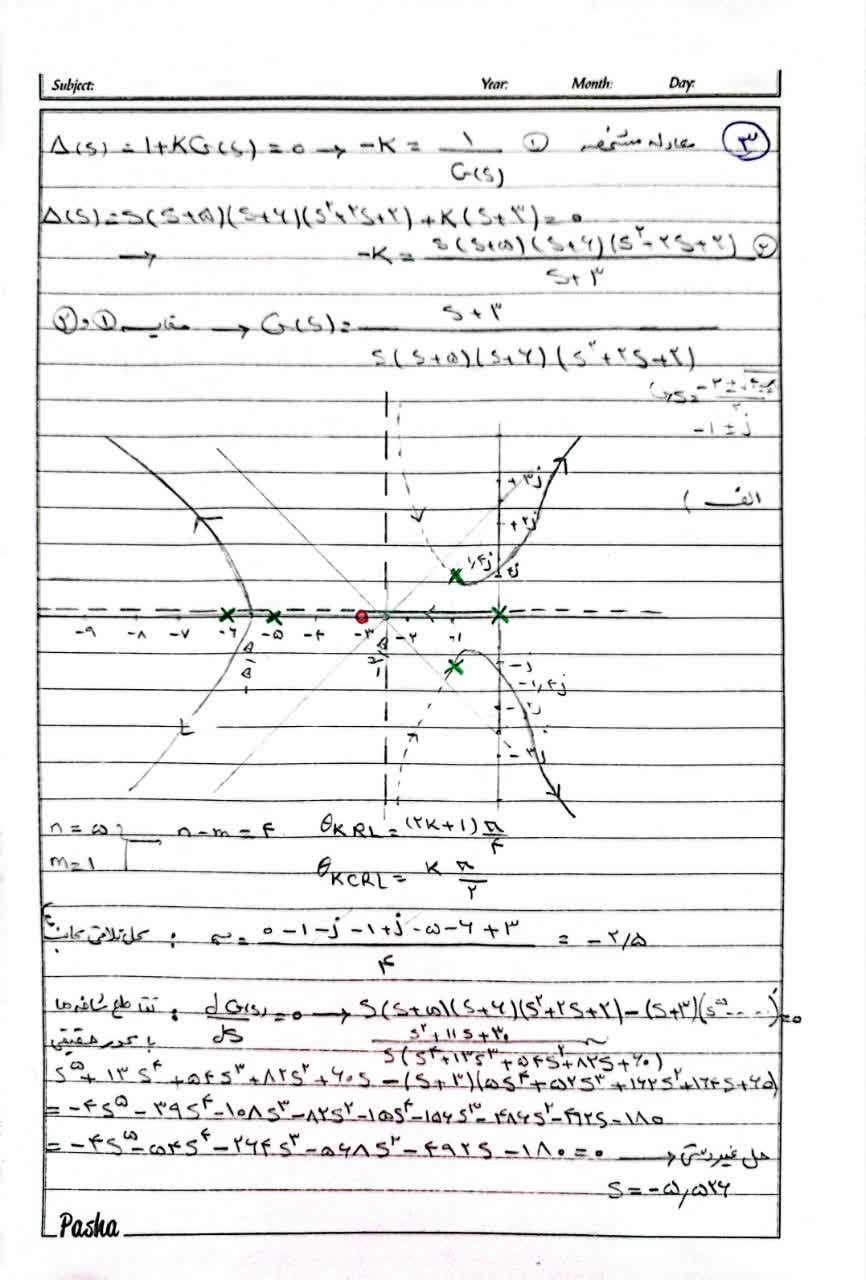
\includegraphics[width=15cm]{q3.jpg}
			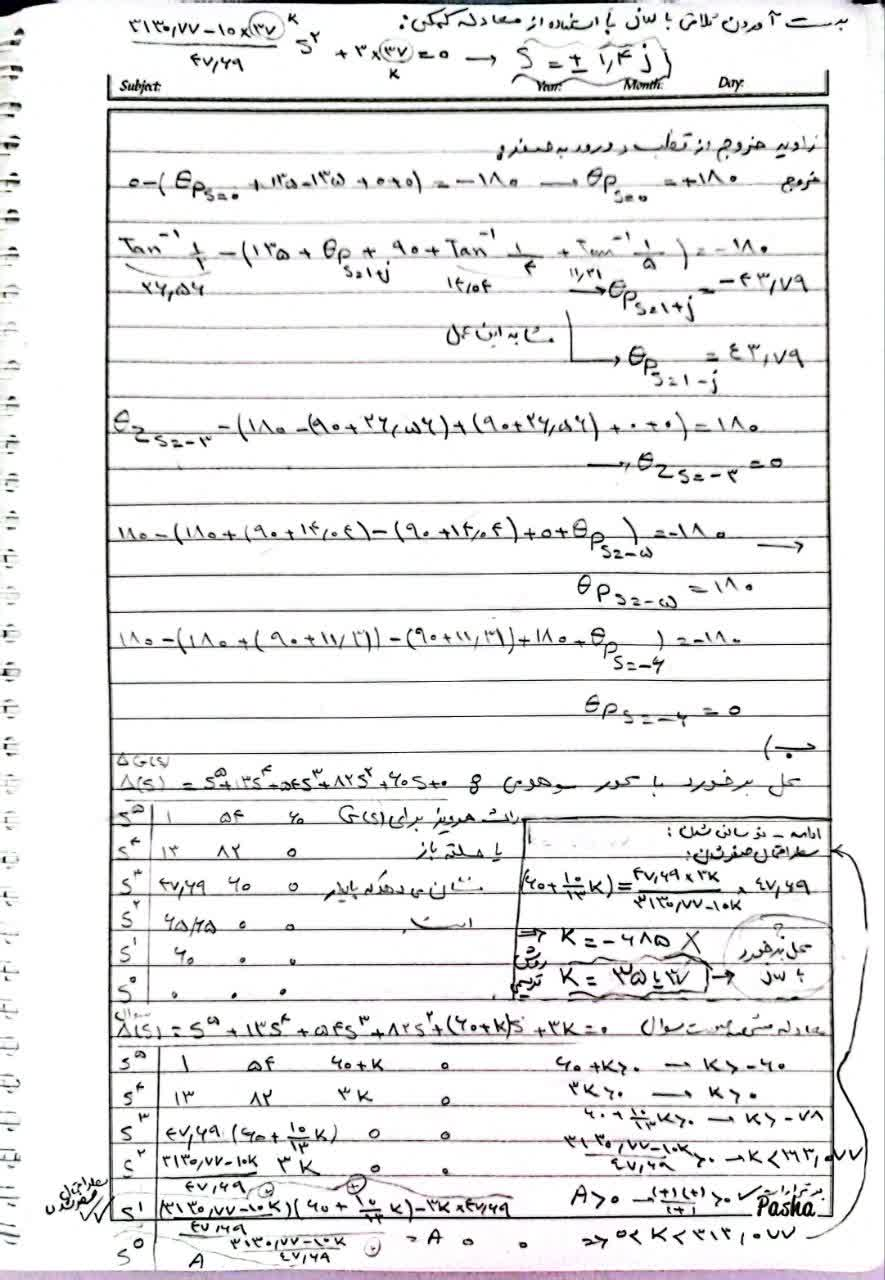
\includegraphics[width=15cm]{q3p.jpg}
			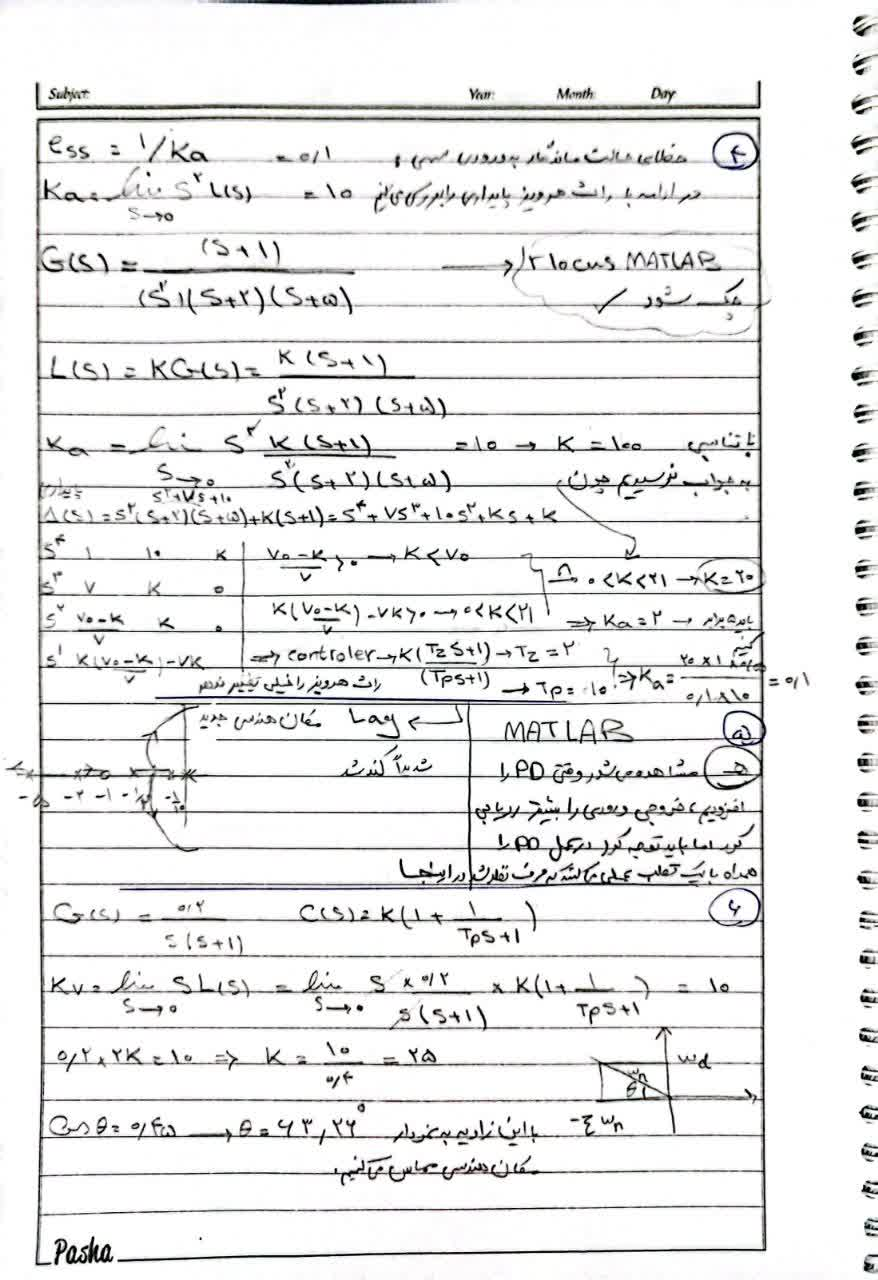
\includegraphics[width=15cm]{q4,5,6.jpg}
			\includegraphics[width=15cm]{q6.jpg}
		
	\section{سوال پنجم}{
         \part{الف}{
         	%% الف
         	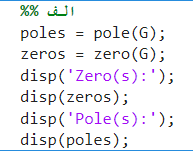
\includegraphics[width=5cm]{Capture.png}
         	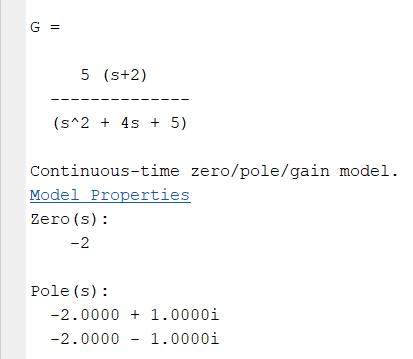
\includegraphics[width=10cm]{output_a.png}
         }
            \part{ب}{
         	%% ب
          	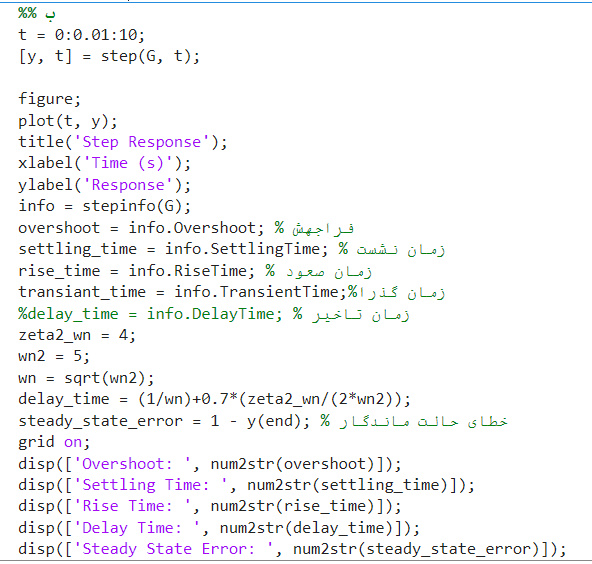
\includegraphics[width=15cm]{Capture1.png}
          	
         	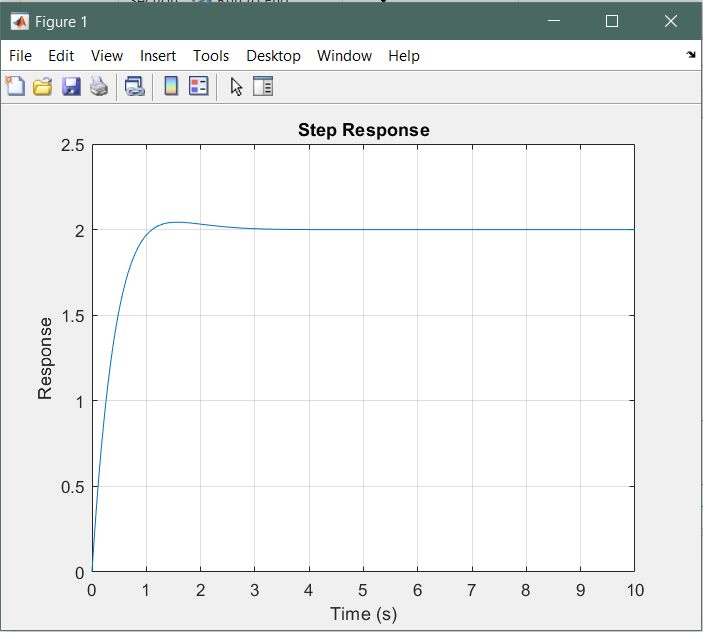
\includegraphics[width=15cm]{Q5_step.png}  \\
         	 توجه : نمودار بالا حلقه باز رسم شده است.\\
         	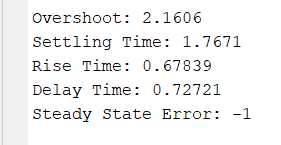
\includegraphics[width=8cm]{output_b.png} 
         }
          \part{ج}{
         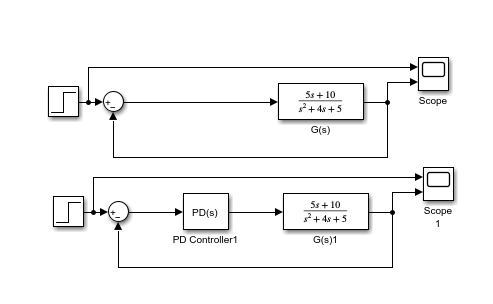
\includegraphics[width=15cm]{Q5.png}
         در ادامه تاثیر اعمال PD بررسی میشود.
         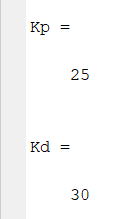
\includegraphics[width=4cm]{Capture2.png}
         }
		    
		\part{د-ه}{
		    توجه : نمودار زیر حلقه بسته رسم شده است.
			\includegraphics[width=15cm]{Q5_without PD.png}
			 نمودار خروجی بدون :PD مشاهده میشود که خروجی به درستی ورودی را ردیابی نمیکند.
			\includegraphics[width=15cm]{Q5_with PD.png}
			 نمودار خروجی با :PD مشاهده میشود که خروجی با تقریب خوبی ورودی را ردیابی میکند.\\
	\part{تحلیل}{
			 اهداف کلی این است که با دادن ورودی پله بتوان خروجی مطلوب را بدست آوریم. با کمک گرفتن از کنترلر PD تواستیم این موضوع را پیگیری کنیم. نکته قابل تتوجه اینست که این جبرانساز در عمل همراه یک قطب اعمال میشود که ما در اینجا صرف نظر کردیم.
			}
			}
	}
	\end{document}